
\documentclass[final]{beamer}

\usepackage[scale=1.24]{beamerposter} % Use the beamerposter package for laying out the poster

\usetheme{confposter} % Use the confposter theme supplied with this template

\usepackage[english]{babel}
\usepackage[latin1]{inputenc}
\usepackage{amsmath, amsthm, amssymb, latexsym}
\usepackage{graphics, graphicx, xcolor}
\usepackage[vcentermath, enableskew]{youngtab}
\usepackage{lipsum,  verbatim}
\usepackage{mathtools}
\usepackage{txfonts}
\usepackage{wrapfig}

\newtheorem{proposition}[theorem]{Proposition}

\theoremstyle{definition}
\newtheorem{remark}[theorem]{Remark}
\numberwithin{equation}{section}

\newcommand{\onep}{1'}
\newcommand{\twop}{2'}
\newcommand{\threep}{3'}
\newcommand{\fourp}{4'}
\newcommand{\fivep}{5'}
\newcommand{\sixp}{6'}
\newcommand{\sevenp}{7'}
\newcommand{\eightp}{8'}
\newcommand{\ninep}{9'}
\newcommand{\iprime}{i'}
\newcommand{\jprime}{j'}
\newcommand{\minustwop}{\textrm{-}2'}
\newcommand{\minusonep}{\textrm{-}1'}
\newcommand{\minustwo}{\textrm{-}2}
\newcommand{\minusone}{\textrm{-}1}
\newcommand{\boldtwo}{\mathbf{2}}
\newcommand{\boldthree}{\mathbf{3}}
\newcommand{\boldtwop}{\mathbf{2'}}
\newcommand{\boldthreep}{\mathbf{3'}}
\newcommand{\boldi}{\boldsymbol{i}}

\newcommand{\wt}{\mathrm{wt}}
\newcommand{\nz}{\mathrm{nz}}

\setbeamercolor{block title}{fg=ngreen,bg=white} % Colors of the block titles
\setbeamercolor{block body}{fg=black,bg=white} % Colors of the body of blocks
\setbeamercolor{block alerted title}{fg=white,bg=dblue!70} % Colors of the highlighted block titles
\setbeamercolor{block alerted body}{fg=black,bg=dblue!10} % Colors of the body of highlighted blocks
% Many more colors are available for use in beamerthemeconfposter.sty

%-----------------------------------------------------------
% Define the column widths and overall poster size
% To set effective sepwid, onecolwid and twocolwid values, first choose how many columns you want and how much separation you want between columns
% In this template, the separation width chosen is 0.024 of the paper width and a 4-column layout
% onecolwid should therefore be (1-(# of columns+1)*sepwid)/# of columns e.g. (1-(4+1)*0.024)/4 = 0.22
% Set twocolwid to be (2*onecolwid)+sepwid = 0.464
% Set threecolwid to be (3*onecolwid)+2*sepwid = 0.708

\newlength{\sepwid}
\newlength{\onecolwid}
\newlength{\twocolwid}
\newlength{\threecolwid}
\setlength{\paperwidth}{48in} % A0 width: 46.8in
\setlength{\paperheight}{36in} % A0 height: 33.1in
\setlength{\sepwid}{0.025\paperwidth} % Separation width (white space) between columns
\setlength{\onecolwid}{0.3\paperwidth} % Width of one column
\setlength{\twocolwid}{0.625\paperwidth} % Width of two columns
\setlength{\threecolwid}{0.95\paperwidth} % Width of three columns
\setlength{\topmargin}{-0.5in} % Reduce the top margin size
%-----------------------------------------------------------

\usepackage{booktabs} % Top and bottom rules for tables

%----------------------------------------------------------------------------------------
%	TITLE SECTION 
%----------------------------------------------------------------------------------------

\title{Type-C Stanley Symmetric Functions and Shifted Primed Tableaux} % Poster title

\author{Graham Hawkes, Kirill Paramonov and Anne Schilling} % Author(s)

\institute{University of California, Davis} % Institution(s)

%----------------------------------------------------------------------------------------

\begin{document}

\addtobeamertemplate{block end}{}{\vspace*{2ex}} % White space under blocks
\addtobeamertemplate{block alerted end}{}{\vspace*{2ex}} % White space under highlighted (alert) blocks

\setlength{\belowcaptionskip}{2ex} % White space under figures
\setlength\belowdisplayshortskip{2ex} % White space under equations

\begin{frame}[t] % The whole poster is enclosed in one beamer frame

\begin{columns}[t] % The whole poster consists of three major columns, the second of which is split into two columns twice - the [t] option aligns each column's content to the top

\begin{column}{\sepwid}\end{column} % Empty spacer column

\begin{column}{\twocolwid}\vspace{-.4in} % The first column

%----------------------------------------------------------------------------------------
%	GOAL
%----------------------------------------------------------------------------------------

\begin{alertblock}{Goal}

It is known that Stanley symmetric functions are Schur-positive, i.e. the coefficients of the Schur expansion are non-negative. 
Our goal here is to introduce a crystal structure on the set of unimodal factorizations that is isomorphic to the crystal structure of type-A crystal.

In particular, we use Kra\'skiewicz insertion to use the notion of Primed Tableaux and introduce crystal operators on those tableaux instead.

\end{alertblock}


%----------------------------------------------------------------------------------------
%	BACKGROUND
%----------------------------------------------------------------------------------------

\begin{columns}[t]

\begin{column}{\onecolwid}\vspace{-.8in}


\begin{block}{Background}

\textbf{Stanley Symmetric Functions}
\begin{itemize}
\item Coxeter group of type $C_n$ is defined to be generated by $\{s_0, s_1, \ldots, s_{n-1}\}$ subject to relations
	\begin{itemize}
	\item $s_i^2 = 1$ for all $i$,  
	\item $s_i s_j = s_j s_i$ provided $|i-j|>1$, 
	\item $s_i s_{i+1} s_i = s_{i+1} s_i s_{i+1}$ for all $i>0$,
	\item $s_0 s_1 s_0 s_1 = s_1 s_0 s_1 s_0$.
	\end{itemize}
\item Each Coxeter group element $w=s_{i_1}\ldots s_{i_l}$ is represented by a word $i_1\ldots i_l$ and many other equivalent words. Among those, the words of shortest length are called \textit{reduced words}.

\item A word $i_1\ldots i_l$ is called unimodal if there exists an index $\nu$ with $i_1 > \ldots > i_\nu < \ldots < i_l$.  \textit{Unimodal factorization} of a Coxeter group element $w$ is a factorization of its reduced word into unimodal factors. Denote the set of unimodal factorizations of $w$ as $U(w)$.

\item For example, given $w=s_2 s_1 s_2 s_0 s_1 s_0$, some of the elements of $U(w)$ are $(212)(0)(10),\ (21)()(201)(0),\ (1)(2101)(0),\ ()(12)(01)(01)$.

\item Given unimodal factorization $\mathbf{A}$, define its \textit{weight} $\wt(\mathbf{A})$ to be the vector 
consisting of the number of elements in each factor, and $\nz(\mathbf{A})$ to be the number of non-empty factors.


\item \textit{Type-C Stanley symmetric function} is defined as 
$$F^C_w(\mathbf{x}) = \sum_{\mathbf{A} \in U(w)} 2^{\nz(\mathbf{A})} \mathbf{x}^{\wt(\mathbf{A})}.$$
\end{itemize}
\vskip 15pt

\begin{wrapfigure}{r}{0.16\textwidth}
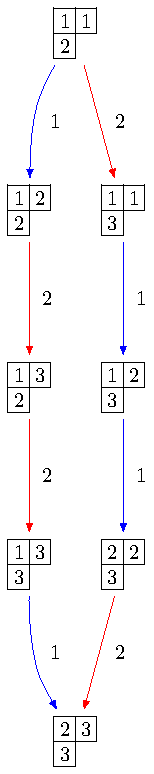
\includegraphics[scale=1.6]{Crystal_Young}
\centering
\end{wrapfigure}

\textbf{Type-A crystals and Schur Functions}\vskip 10pt

An example of a crystal of type $A_2$ is shown to the right.

To define a crystal, one needs to define crystal operators $f_i$, which induce digraph structure, which splits the set into several components.

Each connected component is determined by the highest weight element, and the character of each connected component equal to a symmetric Schur polynomial $s_{\lambda}(x_1,\ldots,x_{n+1})$ with $\lambda\vdash h$.

In the limit $n\to\infty$ Schur polynomials become Schur functions $s_\lambda(\mathbf{x})$. Schur functions form an orthonormal basis to the vector space of symmetric functions with integer coefficients.


\end{block}

%----------------------------------------------------------------------------------------

\end{column} % End of the first column

\begin{column}{\sepwid}\end{column} % Empty spacer column

\begin{column}{\onecolwid}\vspace{-.8in} % The first column within column 2 (column 2.1)


%----------------------------------------------------------------------------------------
%	TABLEAUX
%----------------------------------------------------------------------------------------

\begin{block}{Unimodal Tableaux and Shifted Primed Tableaux}

A \textit{shifted diagram} $\mathcal{S}(\lambda)$ associated to a partition $\lambda = (\lambda_1,\ldots,\lambda_\ell)$ with $\lambda_i > \lambda_{i+1}$ is the set of 
boxes in positions $(i,j)$ satisfying $1\leqslant i\leqslant \ell$ and $ i\leqslant j\leqslant \lambda_i+i-1$.

\textbf{Unimodal Tableaux}
\begin{itemize}

\item A \textit{unimodal tableau} $\mathbf{P}$ of shape $\lambda$ associated to a Coxeter group element $w$ of type $C_n$ is a filling of a shifted diagram $\mathcal{S}(\lambda)$ with letters from the alphabet \small$\{0< 1 < 2< \cdots < n-1\}\ $\normalsize such that
	\begin{itemize}
	\item the rows of $\mathbf{P}$, denoted by $P_1, \ldots, P_\ell$, are unimodal words,
	\item $P_i$ is the longest unimodal subsequence in a concatenated word $P_{i+1}P_i$,
	\item the concatenated word $P_\ell P_{\ell-1} \ldots P_1$ a reduced type-C word that represents $w$.
	\end{itemize}
\item For example, unimodal tableau $\small\young(43201,:212)$ corresponds to $w=s_2 s_1 s_2 s_4 s_3 s_2 s_0 s_1$.
\end{itemize}

\textbf{Primed Tableaux}
\begin{itemize}
\item A \textit{primed tableau} $\mathbf{T}$ of shape $\lambda$ on $n$ letters is a filling of $\mathcal{S}(\lambda)$ 
with letters from the alphabet \small$\{1' < 1 < 2'< 2< \cdots <m' < m\}\ $\normalsize such that:
	\begin{itemize}
	\item The entries are weakly increasing along each column and each row of $\mathbf{T}$.
	\item Each row contains at most one $i'$ for every $i = 1,\ldots,m$.
	\item Each column contains at most one $i$ for every $i = 1,\ldots,m$.
	\end{itemize}
\item The weight of a primed tableau, denoted by $\wt(\mathbf{T})$, is the vector with $i$-th coordinate equal to the total number of letters in $\mathbf{T}$ that are either $i$ or $i'$.
\item For example, $\small\young(11\twop\threep3,:\twop2\threep)$ is a primed tableau of weight $(2,3,3)$.
\end{itemize}

\end{block}

%----------------------------------------------------------------------------------------
%	KR INSERTION
%----------------------------------------------------------------------------------------

\begin{alertblock}{Kra\'skiewicz insertion}

The Kra\'skiewicz insertion gives a bijection 
\begin{equation*}
\mathrm{KR}\colon U^{\pm}(w) \rightarrow \bigcup_{\lambda} \big[\mathcal{UT}_w (\lambda) \times \mathcal{PT}^\pm (\lambda)\big],
\end{equation*}
where $U^{\pm}(w)$ is the set of all unimodal factorizations of $w$ with a sign assigned to each non-zero factor, $\mathcal{UT}_w (\lambda)$ is the set of all unimodal tableaux of shape $\lambda$ associated with $w$, and $\mathcal{PT}^\pm (\lambda)$ is the set of all primed tableaux of shape $\lambda$.

Moreover, the weight of a unimodal factorization is equal to the weight of a primed tableau in the image.

\end{alertblock}

\end{column} % End of column 2.2

\end{columns}

\end{column}

\begin{column}{\sepwid}\end{column} % Empty spacer column

\begin{column}{\onecolwid}\vspace{-.6in} % The third column

%----------------------------------------------------------------------------------------
%	OPERATORS
%----------------------------------------------------------------------------------------

\begin{block}{Lowering operator $f_i$ on Primed Tableau}

We can introduce a crystal structure on the set $\mathcal{PT} (\lambda)$ instead and induce the structure on $U^{\pm}(w)$ via the Kra\'skiewicz insertion. 

In particular, we obtain the Schur expansion of the characteristic function of $\mathcal{PT}^\pm (\lambda)$, also known as $Q$-Schur function, and get the expansion of type-C Stanley symmetric function by summing over all elements of $\mathcal{UT}_w (\lambda)$.

It is convenient to define the crystal operators on the subset of $\mathcal{PT}^\pm (\lambda)$ with no primed elements on the diagonal (denoted by $\mathcal{PT} (\lambda)$), and extend the action on the whole set afterwards. 

Consider a primed tableau $\mathbf{T}$.

\begin{itemize}
\item Construct the \textit{reading word}  $\mathrm{rw}(\mathbf{T})$ as follows:

	\begin{enumerate}
	\item List all primed letters in the tableau, column by column, in decreasing order within each column, moving from the rightmost column to the left, and with all the primes removed.
	\item Then list all unprimed elements, row by row, in increasing order within each row, moving from the bottommost row to the top.
	\end{enumerate}

\item Apply a bracketing rule for letters $i$ and $i+1$ in $\mathrm{rw}(\mathbf{T})$ to find an $i$ that operator $f_i$ would act on. If no such $i$ exist, the operator $f_i$ is not defined for $\mathbf{T}$.

\item As an example, crystal structure for $\mathcal{PT} ((3,1))$ is shown below.
\end{itemize}


\begin{wrapfigure}[26]{l}{0.54\textwidth}
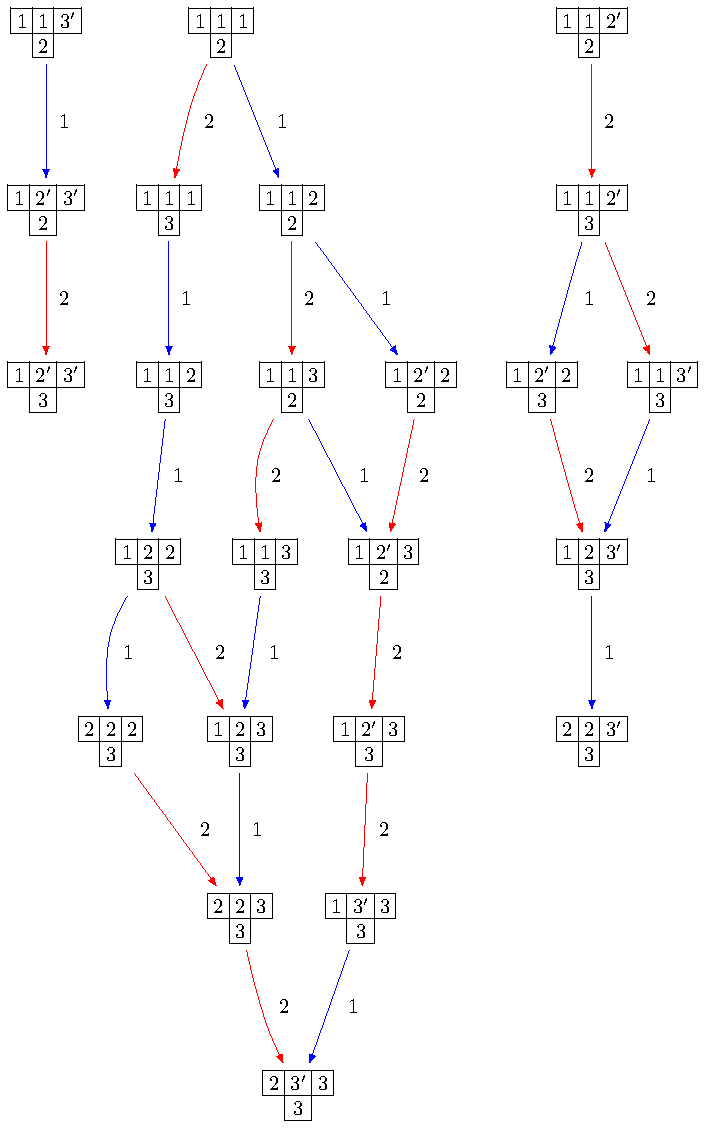
\includegraphics[scale=1.55]{Crystal_Shifted}
\centering
\end{wrapfigure}

 Schur expansion of the characteristic function of $\mathcal{PT} ((3,1))$, also known as $P$-Schur function, is
 \begin{equation*}
 P_{(3,1)} = s_{(2,1,1)} + s_{(3,1)} + s_{(2,2)}.
 \end{equation*}
 
 Characteristic function of $\mathcal{PT}^\pm ((3,1))$ is
 \begin{equation*}
 Q_{(3,1)} = 4 P_{(3,1)}.
 \end{equation*}
 
 And, finally, taking long Coxeter group element $$w=s_0 s_1 s_0 s_1,$$ 
 characteristic function of $U^\pm(w)$
 \begin{equation*}
 F^C_w = 4 s_{(2,1,1)} + 4 s_{(3,1)} + 4 s_{(2,2)},
 \end{equation*}
 since there is only one unimodal tableau corresponding to $w$, namely $$\small\young(101,:0).$$


In general, the highest weight elements of $\mathcal{PT} (\lambda)$ are exactly the ones with Yamanouchi reading words, and Schur expansion of $F^C_w$ can be found similarly.

\end{block}

%----------------------------------------------------------------------------------------

\end{column} % End of the third column

\end{columns} % End of all the columns in the poster

\end{frame} % End of the enclosing frame

\end{document}
